\documentclass[10pt,a4paper]{article}
\usepackage[margin=17mm]{geometry}
\usepackage[T1]{fontenc}
\usepackage{lmodern,amsmath,amssymb,graphicx,booktabs,xcolor,hyperref}
\hypersetup{colorlinks=true,urlcolor=blue,pdftitle={Chained 2-power descent: genus-three boundary}}
\setlength{\parindent}{0pt}
\setlength{\parskip}{5pt}
\setcounter{secnumdepth}{0}
\begin{document}
{\LARGE\bfseries Chained 2-power descent}\par
{\large Genus-three boundary and complete finite validation}\par
23 November 2026 \quad Chained ECDLP Transfers \quad PR 4997

\medskip
\fcolorbox{blue!35!black}{blue!4}{\parbox{0.95\linewidth}{\textbf{Status.}
Two distinct same-author Rust algorithms agree on the complete finite model.
Producer evidence remains unsigned. Both endpoints are product PPAVs;
no genus-three Jacobian transfer or ECDLP advantage is qualified.
\texttt{[pcc:unverified]}}}

\section{A stable composite kernel with no rational first step}
On $A=E^3$, with $E/\mathbb F_5:y^2=x^3+2x+1$, use the product pairing
and the mod-$4$ blocks
\[
 F=\begin{pmatrix}0&3\\1&3\end{pmatrix},\qquad
 M=I+2F=\begin{pmatrix}1&2\\2&3\end{pmatrix},\qquad
 K=E_1[2]\oplus\operatorname{Graph}(M|_{E[4]}).
\]
Native A checks the complete module $(\mathbb Z/4)^6$ and standard alternating
form. The geometric identification on page 2 is a written bridge;
geometric torsion coordinates were not evaluated. \texttt{[pcc:unverified]}

\begin{center}
\begin{tabular}{@{}lr@{}}
\toprule
Observed finite population or invariant & Exact value\\
\midrule
Ambient mod-$4$ vectors & 4,096\\
Kernel $K$; full orthogonal $K^\perp$ & 64; equal\\
$K[2]$; doubled image $2K$ & 16; 4\\
Nonzero fixed vectors in ambient two-torsion & 0\\
All first Lagrangians in $\mathbb F_2^6$ & 135\\
Frobenius-stable first Lagrangians & 0\\
Compatible first kernels $2K\subset L\subset K[2]$ & 3\\
All rank-$3$ subspaces in the second enumeration & 1,395\\
Frobenius-stable rank-$3$ subspaces of any kind & 0\\
\bottomrule
\end{tabular}
\end{center}

\begin{center}
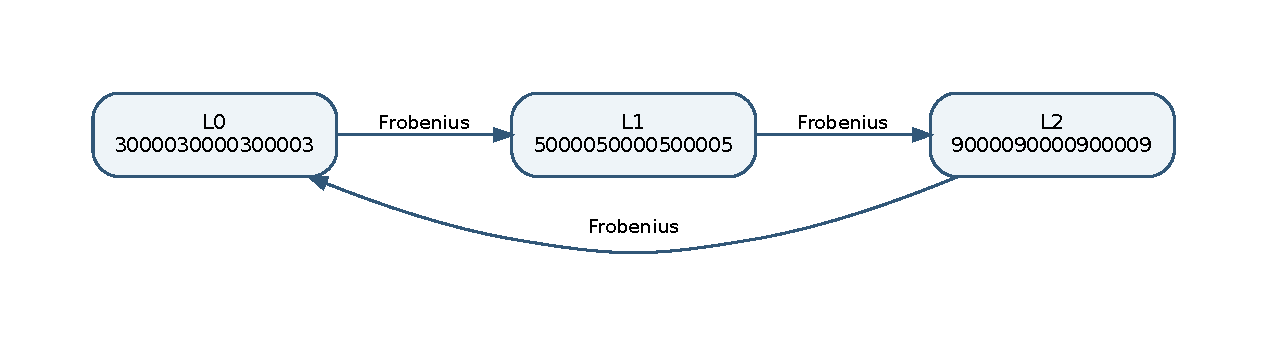
\includegraphics[width=0.94\linewidth]{first-kernel-cycle.pdf}\\[-1mm]
{\small The three compatible first kernels form one Frobenius cycle.
Hexadecimal labels encode complete $64$-bit spans. These arrows act on kernels;
they are not evaluated divisor maps.}
\end{center}

\textbf{Two methods.} A generates independent isotropic triples and deduplicates
their spans. C enumerates canonical RREFs for every rank-$3$ subspace, derives
$K$ from independent linear congruences, and checks a four-generator Gram
certificate. Every published $K$ point, order, Frobenius image, $L$ span and
compatibility flag agrees. The provided summary line is ignored by C.
\texttt{[pcc:unverified]}

\textbf{Controls.} Identity $M$ fails isotropy with pairing $2$ on encoded points
$1088,272$; restoration succeeds. Identity $F$ retains all $135$ Lagrangians.
C rejects corrupted copies of one $L$ image and one $K$ identifier, then
accepts the unchanged original data. \texttt{[pcc:unverified]}

\newpage
{\Large\bfseries Geometry, scope and reproducibility}\par

\section{Written realization and decomposable endpoints}
All $25$ affine pairs on $E/\mathbb F_5$ were checked: $\#E=7$, trace $-1$,
and nonzero discriminant. Standard Frobenius theory gives
$\pi^2+\pi+[5]=0$. Its mod-$2$ polynomial is irreducible, so a primitive
$v\in E[4]$ gives a basis $(v,\pi v)$, producing $F$. The endomorphism
$[1]+[2]\pi$ restricts to $M$; determinant $3$ makes it anti-isometric modulo
$4$. \texttt{[pcc:unverified]}

Standard polarized quotient theory gives a degree-$64$ quotient over
$\mathbb F_5$. Compatible first kernels have orbit length $3$, requiring
$\mathbb F_{125}$; each geometric step has degree $8$. This is a written
quotient/descent argument, not an implemented morphism or shared Lean theorem.
\texttt{[pcc:unverified]}

The source is the product $E^3$, and the polarized target splits as
\[
 (E_1/E_1[2])\ \times\ ((E_2\times E_3)/\operatorname{Graph}(M)).
\]
Neither endpoint provides a smooth genus-$3$ Jacobian with its canonical
principal polarization. On the known $E_1$ factor the quotient identifies
with multiplication by $2$. No explicit divisor images or matched costs
were measured for transfer, solving, recovery, setup, linear algebra and
memory. There is no measured comparison with rho, BSGS or index calculus. \texttt{[pcc:unverified]}

\section{Candidate all-length genus-two reduction}
Over a field of characteristic different from $2$, let $A$ be a principally
polarized abelian surface with $A(k)[2]=0$, and let a rational $2^n$-polarized
kernel be $H$. The stable characteristic layers
$W_j=(2^{j-1}H)[2]\subset A[2]$ have dimension $0,2$ or $4$: a stable line
would give a rational nonzero point, while a stable hyperplane has a stable
perpendicular line. Exponent multiplicities are therefore even. The written
candidate yields
\[
 H\cong(C_{2^a})^2\times(C_{2^b})^2,\quad a\ge b\ge0,\quad a+b=n,\qquad f=h\circ[2^b],
\]
with a rational $(2,2)$ quotient flag for the residual free kernel.
Intermediate products/Weil restrictions remain possible. This extends the
retained CT331 irreducible sector; shared Mathlib, quotient and representation
obligations remain open. \texttt{[pcc:unverified]}

\section{Exact evidence and first failure}
\begin{tabular}{@{}p{0.19\linewidth}p{0.76\linewidth}@{}}
\toprule
A source & \texttt{61f7b10c6dee4bb35768c19824fe326af225e254}\\
A full stdout & 12,324 bytes; SHA-256\\
& \texttt{e89299c3b5a801688f87d7924cae6b06a8288c17cda5ab895b79816047194ed0}\\
C source & \texttt{8a9247c1aa2ef1ce1fa7a4a75d185ee79f435450}\\
C full stdout & 27,359 bytes; SHA-256\\
& \texttt{0e0da3c49d3b06d4ea6e38090e6616c95f23c0995e8f4143a690cb2e60930a51}\\
\bottomrule
\end{tabular}

B compiled, but strict Clippy failed before verification. C preserves that
source and changes only two parity expressions in a new file. A and C each
pass all seven phases with $2$~GiB virtual memory, $120$~seconds per phase
and one worker. Complete source readback and build/pre-call/post-call guards
match. All small raw is retained; whole compiled packets remain private
with remote custody pending. This is not a signed PCC verdict.
\texttt{[pcc:unverified]}

{\footnotesize Full arguments and raw: \path{RESULT_A_AND_GEOMETRIC_SCOPE.md},
\path{CURRENT_RESULT_C.md}, \path{ACTUAL_FIRST_A_RESULT.json},
\path{ACTUAL_FIRST_C_RESULT.json}, and phase directories. Context:
Smith, arXiv:0806.2995v2, \S9; Magma Richelot handbook, text 1615;
Bruin--Doerksen, arXiv:0902.3480. No novelty clearance is claimed.
\url{https://github.com/isogeny-labs/crypto/pull/4997} \quad
\url{https://github.com/isogeny-labs/crypto/issues/3904}.}
\end{document}
